\documentclass{article}
\usepackage{ctex}
\usepackage[english]{babel}
\usepackage{blindtext}
\usepackage{nameref}
\usepackage{fancyhdr}
\usepackage{amsmath,amssymb,amsthm}
\usepackage{graphicx,float}
\usepackage{physics}
\usepackage[a4paper, total={6in, 9in}]{geometry}

\graphicspath{ {../Pictures/} }

\pagestyle{plain}
\fancyhf[CF]{\thepage}

\title{High Level Design Document\\Become Pac-Man\\version: 1}
\author{Group F8\\1155127434 HO Chun Lung Terrance\\
Department of Philosophy, The Chinese University of Hong Kong\\1155143519 WOO Pok\\
Department of Physics, The Chinese University of Hong Kong\\1155157839 NG Yu Chun Thomas\\
Department of Computer Science and Engineering, The Chinese University of Hong Kong\\1155157719 LEUNG Kit Lun Jay\\
Department of Computer Science and Engineering, The Chinese University of Hong Kong\\1155143569 MOK Owen\\
Department of Mathematics, The Chinese University of Hong Kong}
\date{\today}

\begin{document}
\maketitle
\tableofcontents
\newpage
\section{Introduction}
\subsection{Project Overview}
\par This project is to create a Pac-Man game through Unity game engine. The infamous Pac-Man game is one side an arcade game to escape from the chasing of ghosts, but one side has the potential to become a dungeon-like horror game, such as dark deception. We aim at producing a brand-new Pac-Man game inheriting the idea of traditional Pac-Man, but enhancing the experience by introducing horror features. The project will be built under the guidance of software development, and be evaluated by aspects of software engineering taught in the course CSCI3100 Software Engineering.

\subsection{System Feature}
\par The system features:
\begin{enumerate}
    \item 3-D constructions: Apart from traditional Pac-Man games, this project will introduce a 3-D maze with 3-D objects for advanced experience of Pac-Man.
    \item Props: Pac-Man will interact with props inside the maze. When Pac-Man eats special props, there will be buffs or de-buffs according to the function of that prop. Usual beans will be placed as main props.
    \item Third-person camera: The sight of player could no longer be a god view, but focusing on the surrounding of the Pac-Man. Players will eventually experience the feeling of being a Pac-Man.
    \item Teleport: With different levels of the Pac-Man game, the length of the gameplay will be increased by inserting teleports. The teleports may bring players to a specific point, or act as a bridge between mazes.
    \item Fog of war: As difficulties diverges, player may see only the sight of the Pac-Man, but no longer its surrounding. In particular, under the situation of fog, player has no ability to see what's behind the Pac-Man if he isn't facing in that direction.
    \item Artificial intelligence of the ghost: Ghost might move in random direction such that player could easily escape from their chase. However, once the difficulty is being raised, the ghost may have the ability to trace player's movement. They could also reflect from histories to attack the frequently appear spot of the player, so no exact solution could be given to win the game easily.
    \item Store system: As if most of the arcade games, player may buy characters or any items from store to enhance their in-game experience.
\end{enumerate}
\section{System Architecture}
\subsection{Technologies}
\par This project will be produced using the following technologies:
\begin{itemize}
    \item Game Engine: Unity (Version 2021.3.17f1)
    \item Programming language: C\#
    \item Documentation: Markdown, LaTeX, MS Word
    \item Database: Firebase
    \item Graphic Processor: Blender
\end{itemize}
\subsection{Architecture Diagram}
\begin{figure}[H]
    \centering
    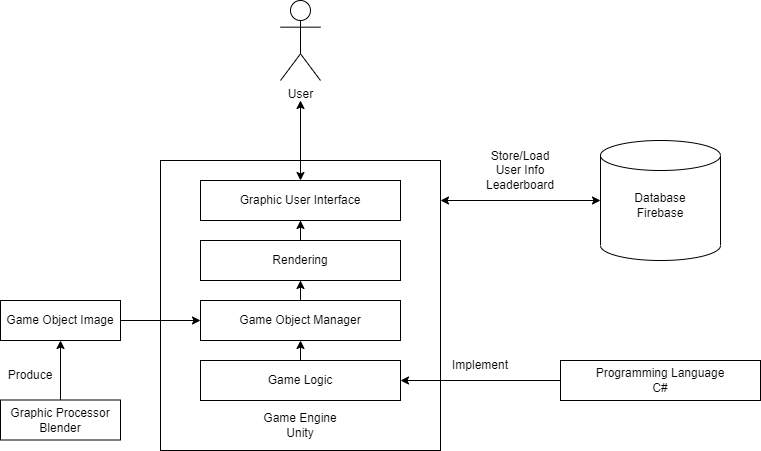
\includegraphics[width=0.8\linewidth]{ArchitectureDiagram.png}
\end{figure}
\subsection{System Components}
\par Unity is a game engine with integrated with multiple components. The designed game logic can be implemented by script created in Unity, which can be edit through external code editor with programming language C\#. Game object manager is also included in Unity to manage and operate the objects, scripts and settings to apply the logic into the program. Sprites, animations or models are needed for the objects to have a image to be rendered and showed in the Graphic User Interface(GUI). The mentioned images can be imported from external graphic processor. e.g. Blender for 3D modeling. And the imported model can be assigned to the corresponding objects through Unity's object manager. The objects then can be rendered by Unity's renderer and displayed as the game window, which is also served as the GUI for users to interact with the game. A database is also needed for the game engine to store user's information from user's input. And the information exchange between the database and game engine can be managed by built-in package of Unity, such that the game engine can store or load user's information or game data with the external database.
\end{document}